\documentclass[12pt, aspectratio=169]{beamer}
\usetheme{moloch}

\molochset{progressbar=head}

\usepackage{appendixnumberbeamer}
\setbeamercovered{transparent=15}
\setbeamertemplate{section in toc}[sections numbered]
\setbeamertemplate{page number in head/foot}[appendixframenumber]

\usepackage{amsmath, mathtools, amssymb}
\usepackage{physics}
\usepackage{tikz}
\usepackage{pgfplots}
\usetikzlibrary{arrows.meta}
\usetikzlibrary{backgrounds}
\usepgfplotslibrary{patchplots}
\usepgfplotslibrary{fillbetween}

\usepackage[
    style=apa
]{biblatex}
\addbibresource{refs.bib}

\title{Irreversible Adaptation and\\Knightian Climate Uncertainty}
\subtitle{\textcite{yan_irreversible_2025}}
\author{Andrea Titton}
\date{\today}

\begin{document}

\maketitle

\section{Model}
\begin{frame}
    \begin{columns}
        \begin{column}{0.6\textwidth}
            \begin{equation*}
                \pi(t) = a_{i(t)} N(t)^{b_{i(t)}}
            \end{equation*} \uncover<2->{where $i(t) = 1$ if the firm has adopted an adaptation technology at time $t$.}
        \end{column}
        \begin{column}{0.4\textwidth}
            \begin{itemize}
                \item Profits $\pi(t)$,
                \item natural resource $N(t)$,
                \item profitability $a_i$,
                \item dependence $b_i$.
            \end{itemize}
        \end{column}
    \end{columns}
\end{frame}

\begin{frame}
    Technology makes the firm \begin{align*}
        \text{more profitable } a_1 &\geq a_0 \\
        \text{less susceptible } b_1 &\leq b_0.
    \end{align*}
    
    \begin{figure}
        % Recommended preamble:
% \usetikzlibrary{arrows.meta}
% \usetikzlibrary{backgrounds}
% \usepgfplotslibrary{patchplots}
% \usepgfplotslibrary{fillbetween}
% \pgfplotsset{%
%     layers/standard/.define layer set={%
%         background,axis background,axis grid,axis ticks,axis lines,axis tick labels,pre main,main,axis descriptions,axis foreground%
%     }{
%         grid style={/pgfplots/on layer=axis grid},%
%         tick style={/pgfplots/on layer=axis ticks},%
%         axis line style={/pgfplots/on layer=axis lines},%
%         label style={/pgfplots/on layer=axis descriptions},%
%         legend style={/pgfplots/on layer=axis descriptions},%
%         title style={/pgfplots/on layer=axis descriptions},%
%         colorbar style={/pgfplots/on layer=axis descriptions},%
%         ticklabel style={/pgfplots/on layer=axis tick labels},%
%         axis background@ style={/pgfplots/on layer=axis background},%
%         3d box foreground style={/pgfplots/on layer=axis foreground},%
%     },
% }

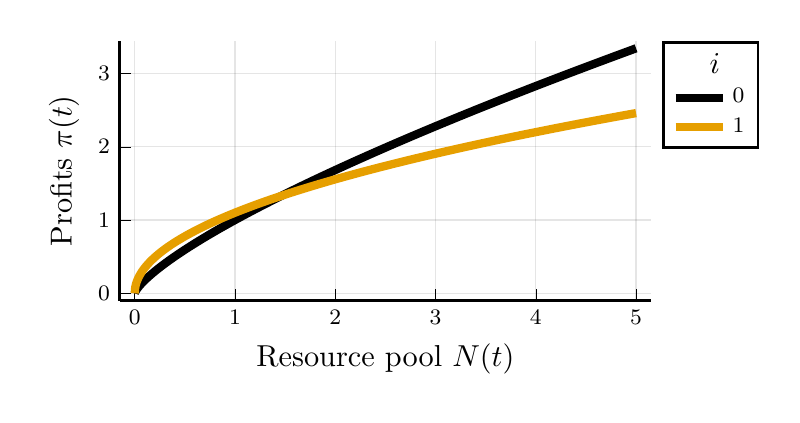
\begin{tikzpicture}[/tikz/background rectangle/.style={fill={rgb,1:red,0.0;green,0.0;blue,0.0}, fill opacity={0.0}, draw opacity={0.0}}, show background rectangle]
\begin{axis}[point meta max={nan}, point meta min={nan}, legend cell align={left}, legend columns={1}, title={}, title style={at={{(0.5,1)}}, anchor={south}, font={{\fontsize{14 pt}{18.2 pt}\selectfont}}, color={rgb,1:red,0.0;green,0.0;blue,0.0}, draw opacity={1.0}, rotate={0.0}, align={center}}, legend style={color={rgb,1:red,0.0;green,0.0;blue,0.0}, draw opacity={1.0}, line width={1}, solid, fill={rgb,1:red,0.0;green,0.0;blue,0.0}, fill opacity={0.0}, text opacity={1.0}, font={{\fontsize{8 pt}{10.4 pt}\selectfont}}, text={rgb,1:red,0.0;green,0.0;blue,0.0}, cells={anchor={center}}, at={(1.02, 1)}, anchor={north west}}, axis background/.style={fill={rgb,1:red,0.0;green,0.0;blue,0.0}, opacity={0.0}}, anchor={north west}, xshift={1.0mm}, yshift={-1.0mm}, width={83.3111111111111mm}, height={48.8mm}, scaled x ticks={false}, xlabel={Resource pool $N(t)$}, x tick style={color={rgb,1:red,0.0;green,0.0;blue,0.0}, opacity={1.0}}, x tick label style={color={rgb,1:red,0.0;green,0.0;blue,0.0}, opacity={1.0}, rotate={0}}, xlabel style={at={(ticklabel cs:0.5)}, anchor=near ticklabel, at={{(ticklabel cs:0.5)}}, anchor={near ticklabel}, font={{\fontsize{11 pt}{14.3 pt}\selectfont}}, color={rgb,1:red,0.0;green,0.0;blue,0.0}, draw opacity={1.0}, rotate={0.0}}, xmajorgrids={true}, xmin={-0.15000000000000036}, xmax={5.15}, xticklabels={{$0$,$1$,$2$,$3$,$4$,$5$}}, xtick={{0.0,1.0,2.0,3.0,4.0,5.0}}, xtick align={inside}, xticklabel style={font={{\fontsize{8 pt}{10.4 pt}\selectfont}}, color={rgb,1:red,0.0;green,0.0;blue,0.0}, draw opacity={1.0}, rotate={0.0}}, x grid style={color={rgb,1:red,0.0;green,0.0;blue,0.0}, draw opacity={0.1}, line width={0.5}, solid}, axis x line*={left}, x axis line style={color={rgb,1:red,0.0;green,0.0;blue,0.0}, draw opacity={1.0}, line width={1}, solid}, scaled y ticks={false}, ylabel={Profits $\pi(t)$}, y tick style={color={rgb,1:red,0.0;green,0.0;blue,0.0}, opacity={1.0}}, y tick label style={color={rgb,1:red,0.0;green,0.0;blue,0.0}, opacity={1.0}, rotate={0}}, ylabel style={at={(ticklabel cs:0.5)}, anchor=near ticklabel, at={{(ticklabel cs:0.5)}}, anchor={near ticklabel}, font={{\fontsize{11 pt}{14.3 pt}\selectfont}}, color={rgb,1:red,0.0;green,0.0;blue,0.0}, draw opacity={1.0}, rotate={0.0}}, ymajorgrids={true}, ymin={-0.10031104574646332}, ymax={3.4440125706285736}, yticklabels={{$0$,$1$,$2$,$3$}}, ytick={{0.0,1.0,2.0,3.0}}, ytick align={inside}, yticklabel style={font={{\fontsize{8 pt}{10.4 pt}\selectfont}}, color={rgb,1:red,0.0;green,0.0;blue,0.0}, draw opacity={1.0}, rotate={0.0}}, y grid style={color={rgb,1:red,0.0;green,0.0;blue,0.0}, draw opacity={0.1}, line width={0.5}, solid}, axis y line*={left}, y axis line style={color={rgb,1:red,0.0;green,0.0;blue,0.0}, draw opacity={1.0}, line width={1}, solid}, colorbar={false}]
    [\addlegendimage{empty legend}] \addlegendentry[font={{\fontsize{11 pt}{14.3 pt}\selectfont}}, text={rgb,1:red,0.0;green,0.0;blue,0.0}] {\hspace{-.6cm}{\textbf{$i$}}}
    \addplot[color={rgb,1:red,0.0;green,0.0;blue,0.0}, name path={45}, draw opacity={1.0}, line width={3}, solid]
        table[row sep={\\}]
        {
            \\
            0.0  0.0  \\
            0.005  0.018803015465431967  \\
            0.01  0.03162277660168379  \\
            0.015  0.042861606445481995  \\
            0.02  0.053182958969449884  \\
            0.025  0.06287167148414677  \\
            0.03  0.07208434242404263  \\
            0.035  0.08091909803534886  \\
            0.04  0.08944271909999159  \\
            0.045  0.09770333436489459  \\
            0.05  0.10573712634405642  \\
            0.055  0.1135721943942021  \\
            0.06  0.12123093028059741  \\
            0.065  0.1287315556465335  \\
            0.07  0.13608915892697748  \\
            0.075  0.14331641883065502  \\
            0.08  0.15042412372345573  \\
            0.085  0.15742155364845226  \\
            0.09  0.16431676725154984  \\
            0.095  0.1711168212482415  \\
            0.1  0.1778279410038923  \\
            0.105  0.18445565501399316  \\
            0.11  0.19100490227716513  \\
            0.115  0.19748011900687698  \\
            0.12  0.2038853093816547  \\
            0.125  0.21022410381342863  \\
            0.13  0.2164998073464082  \\
            0.135  0.22271544017278946  \\
            0.14  0.22887377179317683  \\
            0.145  0.23497735000955589  \\
            0.15  0.2410285256833955  \\
            0.155  0.24702947399772265  \\
            0.16  0.25298221281347033  \\
            0.165  0.25888861859542356  \\
            0.17  0.26475044029330763  \\
            0.175  0.2705693114928809  \\
            0.18  0.2763467610958144  \\
            0.185  0.28208422274232975  \\
            0.19  0.28778304315451386  \\
            0.195  0.2934444895490398  \\
            0.2  0.29906975624424414  \\
            0.205  0.3046599705670381  \\
            0.21  0.3102161981490854  \\
            0.215  0.3157394476884046  \\
            0.22  0.32123067524150845  \\
            0.225  0.3266907881019647  \\
            0.23  0.33212064831351956  \\
            0.235  0.3375210758593954  \\
            0.24  0.34289285156385596  \\
            0.245  0.3482367197374408  \\
            0.25  0.3535533905932738  \\
            0.255  0.35884354245843203  \\
            0.26  0.3641078238014289  \\
            0.265  0.3693468550943378  \\
            0.27  0.37456123052590357  \\
            0.275  0.379751519580101  \\
            0.28  0.38491826849295824  \\
            0.285  0.39006200159903576  \\
            0.29  0.39518322257770583  \\
            0.295  0.4002824156082842  \\
            0.3  0.4053600464421103  \\
            0.305  0.41041656339882987  \\
            0.31  0.41545239829339137  \\
            0.315  0.4204679672996134  \\
            0.32  0.42546367175559907  \\
            0.325  0.4304398989157603  \\
            0.33  0.43539702265375557  \\
            0.335  0.44033540412024136  \\
            0.34  0.4452553923589699  \\
            0.345  0.4501573248844453  \\
            0.35  0.4550415282240584  \\
            0.355  0.45990831842735835  \\
            0.36  0.46475800154489  \\
            0.365  0.46959087407881017  \\
            0.37  0.47440722340731084  \\
            0.375  0.47920732818470435  \\
            0.38  0.4839914587188715  \\
            0.385  0.48875987732763415  \\
            0.39  0.4935128386754873  \\
            0.395  0.4982505900920104  \\
            0.4  0.5029733718731741  \\
            0.405  0.5076814175666632  \\
            0.41  0.512374954242249  \\
            0.415  0.5170542027481706  \\
            0.42  0.5217193779544038  \\
            0.425  0.5263706889836407  \\
            0.43  0.5310083394307343  \\
            0.435  0.5356325275713154  \\
            0.44  0.5402434465602292  \\
            0.445  0.5448412846204029  \\
            0.45  0.549426225222706  \\
            0.455  0.5539984472573267  \\
            0.46  0.5585581251971565  \\
            0.465  0.5631054292536356  \\
            0.47  0.5676405255254853  \\
            0.475  0.5721635761407246  \\
            0.48  0.576674739392341  \\
            0.485  0.5811741698679621  \\
            0.49  0.5856620185738529  \\
            0.495  0.5901384330535419  \\
            0.5  0.5946035575013605  \\
            0.505  0.5990575328711637  \\
            0.51  0.6035004969804791  \\
            0.515  0.6079325846103238  \\
            0.52  0.6123539276009055  \\
            0.525  0.6167646549434175  \\
            0.53  0.6211648928681236  \\
            0.535  0.6255547649289137  \\
            0.54  0.629934392084505  \\
            0.545  0.6343038927764516  \\
            0.55  0.6386633830041155  \\
            0.555  0.643012976396744  \\
            0.56  0.6473527842827909  \\
            0.565  0.6516829157566083  \\
            0.57  0.6560034777426357  \\
            0.575  0.660314575057195  \\
            0.58  0.6646163104680073  \\
            0.585  0.6689087847515286  \\
            0.59  0.6731920967482075  \\
            0.595  0.6774663434157523  \\
            0.6  0.6817316198804996  \\
            0.605  0.6859880194869641  \\
            0.61  0.6902356338456498  \\
            0.615  0.6944745528791982  \\
            0.62  0.6987048648669424  \\
            0.625  0.7029266564879364  \\
            0.63  0.7071400128625219  \\
            0.635  0.7113450175924957  \\
            0.64  0.7155417527999327  \\
            0.645  0.7197302991647223  \\
            0.65  0.7239107359608682  \\
            0.655  0.7280831410916034  \\
            0.66  0.7322475911233668  \\
            0.665  0.7364041613186865  \\
            0.67  0.7405529256680135  \\
            0.675  0.7446939569205465  \\
            0.68  0.7488273266140879  \\
            0.685  0.7529531051039664  \\
            0.69  0.7570713615910637  \\
            0.695  0.7611821641489795  \\
            0.7  0.7652855797503654  \\
            0.705  0.7693816742924606  \\
            0.71  0.7734705126218591  \\
            0.715  0.7775521585585352  \\
            0.72  0.7816266749191567  \\
            0.725  0.7856941235397094  \\
            0.73  0.7897545652974598  \\
            0.735  0.7938080601322794  \\
            0.74  0.7978546670673515  \\
            0.745  0.8018944442292855  \\
            0.75  0.8059274488676564  \\
            0.755  0.8099537373739931  \\
            0.76  0.8139733653002305  \\
            0.765  0.8179863873766472  \\
            0.77  0.8219928575293057  \\
            0.775  0.8259928288970109  \\
            0.78  0.829986353847804  \\
            0.785  0.8339734839950081  \\
            0.79  0.837954270212839  \\
            0.795  0.8419287626515967  \\
            0.8  0.8458970107524514  \\
            0.805  0.8498590632618365  \\
            0.81  0.8538149682454624  \\
            0.815  0.8577647731019631  \\
            0.82  0.8617085245761864  \\
            0.825  0.8656462687721407  \\
            0.83  0.869578051165608  \\
            0.835  0.8735039166164353  \\
            0.84  0.8774239093805121  \\
            0.845  0.8813380731214455  \\
            0.85  0.8852464509219427  \\
            0.855  0.8891490852949078  \\
            0.86  0.8930460181942644  \\
            0.865  0.89693729102551  \\
            0.87  0.9008229446560111  \\
            0.875  0.9047030194250485  \\
            0.88  0.9085775551536168  \\
            0.885  0.9124465911539891  \\
            0.89  0.9163101662390513  \\
            0.895  0.9201683187314137  \\
            0.9  0.9240210864723069  \\
            0.905  0.9278685068302676  \\
            0.91  0.9317106167096201  \\
            0.915  0.9355474525587606  \\
            0.92  0.9393790503782488  \\
            0.925  0.9432054457287128  \\
            0.93  0.9470266737385726  \\
            0.935  0.9508427691115873  \\
            0.94  0.9546537661342304  \\
            0.945  0.9584596986828993  \\
            0.95  0.9622606002309622  \\
            0.955  0.9660565038556471  \\
            0.96  0.9698474422447793  \\
            0.965  0.973633447703367  \\
            0.97  0.9774145521600454  \\
            0.975  0.9811907871733767  \\
            0.98  0.9849621839380145  \\
            0.985  0.9887287732907346  \\
            0.99  0.992490585716335  \\
            0.995  0.9962476513534098  \\
            1.0  1.0  \\
            1.005  1.003747661119124  \\
            1.01  1.0074906638441916  \\
            1.015  1.0112290369843033  \\
            1.02  1.0149628090294402  \\
            1.025  1.018692008155544  \\
            1.03  1.0224166622294937  \\
            1.035  1.0261367988139778  \\
            1.04  1.029852445172268  \\
            1.045  1.0335636282728946  \\
            1.05  1.0372703747942278  \\
            1.055  1.040972711128964  \\
            1.06  1.0446706633885257  \\
            1.065  1.0483642574073684  \\
            1.07  1.0520535187472073  \\
            1.075  1.0557384727011538  \\
            1.08  1.0594191442977763  \\
            1.085  1.063095558305076  \\
            1.09  1.0667677392343893  \\
            1.095  1.07043571134421  \\
            1.1  1.0740994986439416  \\
            1.105  1.0777591248975729  \\
            1.11  1.0814146136272869  \\
            1.115  1.085065988116997  \\
            1.12  1.0887132714158199  \\
            1.125  1.0923564863414776  \\
            1.13  1.0959956554836408  \\
            1.135  1.0996308012072042  \\
            1.14  1.1032619456555044  \\
            1.145  1.1068891107534764  \\
            1.15  1.1105123182107504  \\
            1.155  1.1141315895246935  \\
            1.16  1.1177469459833942  \\
            1.165  1.121358408668593  \\
            1.17  1.1249659984585578  \\
            1.175  1.1285697360309108  \\
            1.18  1.1321696418653988  \\
            1.185  1.13576573624662  \\
            1.19  1.139358039266696  \\
            1.195  1.142946570827901  \\
            1.2  1.1465313506452401  \\
            1.205  1.150112398248986  \\
            1.21  1.1536897329871667  \\
            1.215  1.1572633740280138  \\
            1.22  1.1608333403623647  \\
            1.225  1.164399650806025  \\
            1.23  1.167962324002088  \\
            1.235  1.1715213784232172  \\
            1.24  1.1750768323738858  \\
            1.245  1.1786287039925814  \\
            1.25  1.1821770112539698  \\
            1.255  1.1857217719710247  \\
            1.26  1.1892630037971206  \\
            1.265  1.1928007242280882  \\
            1.27  1.1963349506042402  \\
            1.275  1.1998657001123572  \\
            1.28  1.2033929897876459  \\
            1.285  1.2069168365156608  \\
            1.29  1.210437257034197  \\
            1.295  1.2139542679351496  \\
            1.3  1.2174678856663446  \\
            1.305  1.220978126533338  \\
            1.31  1.2244850067011877  \\
            1.315  1.2279885421961936  \\
            1.32  1.2314887489076136  \\
            1.325  1.234985642589349  \\
            1.33  1.2384792388616033  \\
            1.335  1.241969553212515  \\
            1.34  1.245456600999766  \\
            1.345  1.2489403974521605  \\
            1.35  1.2524209576711833  \\
            1.355  1.2558982966325305  \\
            1.36  1.259372429187618  \\
            1.365  1.2628433700650652  \\
            1.37  1.2663111338721573  \\
            1.375  1.2697757350962822  \\
            1.38  1.2732371881063482  \\
            1.385  1.2766955071541786  \\
            1.39  1.2801507063758828  \\
            1.395  1.2836027997932116  \\
            1.4  1.2870518013148857  \\
            1.405  1.2904977247379101  \\
            1.41  1.2939405837488622  \\
            1.415  1.2973803919251672  \\
            1.42  1.3008171627363485  \\
            1.425  1.304250909545264  \\
            1.43  1.3076816456093203  \\
            1.435  1.3111093840816714  \\
            1.44  1.3145341380123987  \\
            1.445  1.3179559203496731  \\
            1.45  1.3213747439409014  \\
            1.455  1.3247906215338543  \\
            1.46  1.3282035657777793  \\
            1.465  1.331613589224496  \\
            1.47  1.3350207043294777  \\
            1.475  1.3384249234529146  \\
            1.48  1.3418262588607637  \\
            1.485  1.3452247227257832  \\
            1.49  1.3486203271285517  \\
            1.495  1.3520130840584732  \\
            1.5  1.3554030054147672  \\
            1.505  1.3587901030074465  \\
            1.51  1.3621743885582789  \\
            1.515  1.3655558737017361  \\
            1.52  1.368934569985932  \\
            1.525  1.3723104888735425  \\
            1.53  1.3756836417427178  \\
            1.535  1.3790540398879783  \\
            1.54  1.382421694521101  \\
            1.545  1.3857866167719906  \\
            1.55  1.3891488176895423  \\
            1.555  1.392508308242489  \\
            1.56  1.3958650993202388  \\
            1.565  1.3992192017337024  \\
            1.57  1.4025706262161068  \\
            1.575  1.4059193834237984  \\
            1.58  1.4092654839370375  \\
            1.585  1.4126089382607794  \\
            1.59  1.4159497568254462  \\
            1.595  1.419287949987689  \\
            1.6  1.4226235280311383  \\
            1.605  1.4259565011671458  \\
            1.61  1.429286879535516  \\
            1.615  1.4326146732052278  \\
            1.62  1.435939892175147  \\
            1.625  1.439262546374729  \\
            1.63  1.4425826456647133  \\
            1.635  1.445900199837808  \\
            1.64  1.4492152186193652  \\
            1.645  1.4525277116680488  \\
            1.65  1.4558376885764932  \\
            1.655  1.4591451588719522  \\
            1.66  1.4624501320169419  \\
            1.665  1.4657526174098738  \\
            1.67  1.46905262438568  \\
            1.675  1.4723501622164312  \\
            1.68  1.4756452401119453  \\
            1.685  1.4789378672203908  \\
            1.69  1.4822280526288794  \\
            1.695  1.4855158053640545  \\
            1.7  1.48880113439267  \\
            1.705  1.4920840486221618  \\
            1.71  1.4953645569012144  \\
            1.715  1.4986426680203184  \\
            1.72  1.501918390712321  \\
            1.725  1.5051917336529714  \\
            1.73  1.508462705461458  \\
            1.735  1.5117313147009397  \\
            1.74  1.51499756987907  \\
            1.745  1.5182614794485163  \\
            1.75  1.5215230518074698  \\
            1.755  1.5247822953001537  \\
            1.76  1.528039218217321  \\
            1.765  1.5312938287967477  \\
            1.77  1.5345461352237222  \\
            1.775  1.5377961456315252  \\
            1.78  1.541043868101907  \\
            1.785  1.5442893106655562  \\
            1.79  1.5475324813025664  \\
            1.795  1.5507733879428935  \\
            1.8  1.5540120384668108  \\
            1.805  1.5572484407053566  \\
            1.81  1.5604826024407774  \\
            1.815  1.563714531406966  \\
            1.82  1.5669442352898943  \\
            1.825  1.5701717217280404  \\
            1.83  1.5733969983128127  \\
            1.835  1.5766200725889659  \\
            1.84  1.5798409520550158  \\
            1.845  1.5830596441636462  \\
            1.85  1.5862761563221133  \\
            1.855  1.5894904958926435  \\
            1.86  1.5927026701928295  \\
            1.865  1.5959126864960185  \\
            1.87  1.5991205520316982  \\
            1.875  1.6023262739858777  \\
            1.88  1.6055298595014644  \\
            1.885  1.6087313156786367  \\
            1.89  1.6119306495752108  \\
            1.895  1.615127868207007  \\
            1.9  1.6183229785482074  \\
            1.905  1.6215159875317144  \\
            1.91  1.6247069020495  \\
            1.915  1.627895728952956  \\
            1.92  1.6310824750532376  \\
            1.925  1.6342671471216035  \\
            1.93  1.6374497518897526  \\
            1.935  1.6406302960501578  \\
            1.94  1.643808786256394  \\
            1.945  1.6469852291234652  \\
            1.95  1.6501596312281255  \\
            1.955  1.6533319991091988  \\
            1.96  1.6565023392678924  \\
            1.965  1.659670658168111  \\
            1.97  1.6628369622367627  \\
            1.975  1.6660012578640664  \\
            1.98  1.6691635514038512  \\
            1.985  1.6723238491738572  \\
            1.99  1.6754821574560295  \\
            1.995  1.6786384824968104  \\
            2.0  1.681792830507429  \\
            2.005  1.6849452076641875  \\
            2.01  1.6880956201087431  \\
            2.015  1.6912440739483896  \\
            2.02  1.6943905752563317  \\
            2.025  1.6975351300719628  \\
            2.03  1.7006777444011332  \\
            2.035  1.7038184242164205  \\
            2.04  1.7069571754573936  \\
            2.045  1.7100940040308767  \\
            2.05  1.7132289158112095  \\
            2.055  1.7163619166405037  \\
            2.06  1.7194930123288983  \\
            2.065  1.7226222086548117  \\
            2.07  1.725749511365192  \\
            2.075  1.728874926175762  \\
            2.08  1.7319984587712656  \\
            2.085  1.735120114805709  \\
            2.09  1.7382398999025999  \\
            2.095  1.7413578196551858  \\
            2.1  1.7444738796266863  \\
            2.105  1.747588085350528  \\
            2.11  1.7507004423305728  \\
            2.115  1.7538109560413464  \\
            2.12  1.756919631928262  \\
            2.125  1.7600264754078463  \\
            2.13  1.763131491867957  \\
            2.135  1.7662346866680045  \\
            2.14  1.7693360651391663  \\
            2.145  1.7724356325846014  \\
            2.15  1.7755333942796636  \\
            2.155  1.7786293554721115  \\
            2.16  1.7817235213823157  \\
            2.165  1.7848158972034645  \\
            2.17  1.7879064881017694  \\
            2.175  1.7909952992166662  \\
            2.18  1.7940823356610147  \\
            2.185  1.7971676025212964  \\
            2.19  1.8002511048578125  \\
            2.195  1.8033328477048758  \\
            2.2  1.8064128360710052  \\
            2.205  1.8094910749391135  \\
            2.21  1.812567569266699  \\
            2.215  1.8156423239860304  \\
            2.22  1.8187153440043327  \\
            2.225  1.8217866342039692  \\
            2.23  1.824856199442625  \\
            2.235  1.8279240445534854  \\
            2.24  1.8309901743454147  \\
            2.245  1.834054593603131  \\
            2.25  1.8371173070873836  \\
            2.255  1.8401783195351238  \\
            2.26  1.8432376356596771  \\
            2.265  1.8462952601509142  \\
            2.27  1.849351197675416  \\
            2.275  1.8524054528766443  \\
            2.28  1.8554580303751043  \\
            2.285  1.8585089347685089  \\
            2.29  1.8615581706319404  \\
            2.295  1.8646057425180116  \\
            2.3  1.8676516549570246  \\
            2.305  1.8706959124571287  \\
            2.31  1.8737385195044753  \\
            2.315  1.8767794805633746  \\
            2.32  1.879818800076447  \\
            2.325  1.8828564824647764  \\
            2.33  1.8858925321280593  \\
            2.335  1.8889269534447555  \\
            2.34  1.8919597507722343  \\
            2.345  1.8949909284469224  \\
            2.35  1.8980204907844473  \\
            2.355  1.9010484420797833  \\
            2.36  1.9040747866073913  \\
            2.365  1.9070995286213628  \\
            2.37  1.910122672355557  \\
            2.375  1.9131442220237422  \\
            2.38  1.9161641818197312  \\
            2.385  1.9191825559175184  \\
            2.39  1.9221993484714153  \\
            2.395  1.9252145636161824  \\
            2.4  1.928228205467164  \\
            2.405  1.9312402781204188  \\
            2.41  1.9342507856528497  \\
            2.415  1.9372597321223328  \\
            2.42  1.940267121567847  \\
            2.425  1.9432729580095993  \\
            2.43  1.946277245449151  \\
            2.435  1.949279987869542  \\
            2.44  1.9522811892354153  \\
            2.445  1.9552808534931385  \\
            2.45  1.9582789845709268  \\
            2.455  1.9612755863789602  \\
            2.46  1.9642706628095066  \\
            2.465  1.9672642177370376  \\
            2.47  1.9702562550183473  \\
            2.475  1.9732467784926668  \\
            2.48  1.9762357919817812  \\
            2.485  1.979223299290143  \\
            2.49  1.9822093042049864  \\
            2.495  1.9851938104964368  \\
            2.5  1.9881768219176266  \\
            2.505  1.991158342204802  \\
            2.51  1.9941383750774342  \\
            2.515  1.9971169242383275  \\
            2.52  2.0000939933737265  \\
            2.525  2.003069586153425  \\
            2.53  2.006043706230868  \\
            2.535  2.009016357243261  \\
            2.54  2.0119875428116707  \\
            2.545  2.0149572665411295  \\
            2.55  2.0179255320207394  \\
            2.555  2.02089234282377  \\
            2.56  2.0238577025077626  \\
            2.565  2.0268216146146276  \\
            2.57  2.029784082670745  \\
            2.575  2.0327451101870624  \\
            2.58  2.0357047006591906  \\
            2.585  2.0386628575675028  \\
            2.59  2.041619584377229  \\
            2.595  2.044574884538551  \\
            2.6  2.0475287614866966  \\
            2.605  2.0504812186420334  \\
            2.61  2.0534322594101604  \\
            2.615  2.0563818871820025  \\
            2.62  2.0593301053338986  \\
            2.625  2.062276917227693  \\
            2.63  2.0652223262108276  \\
            2.635  2.068166335616427  \\
            2.64  2.0711089487633885  \\
            2.645  2.07405016895647  \\
            2.65  2.0769899994863774  \\
            2.655  2.079928443629849  \\
            2.66  2.082865504649742  \\
            2.665  2.085801185795117  \\
            2.67  2.088735490301323  \\
            2.675  2.0916684213900787  \\
            2.68  2.0945999822695582  \\
            2.685  2.0975301761344705  \\
            2.69  2.1004590061661426  \\
            2.695  2.103386475532599  \\
            2.7  2.1063125873886444  \\
            2.705  2.109237344875939  \\
            2.71  2.112160751123082  \\
            2.715  2.115082809245687  \\
            2.72  2.118003522346461  \\
            2.725  2.1209228935152797  \\
            2.73  2.123840925829267  \\
            2.735  2.1267576223528684  \\
            2.74  2.1296729861379275  \\
            2.745  2.13258702022376  \\
            2.75  2.135499727637228  \\
            2.755  2.1384111113928146  \\
            2.76  2.1413211744926954  \\
            2.765  2.1442299199268122  \\
            2.77  2.1471373506729434  \\
            2.775  2.150043469696777  \\
            2.78  2.1529482799519806  \\
            2.785  2.1558517843802716  \\
            2.79  2.158753985911486  \\
            2.795  2.16165488746365  \\
            2.8  2.164554491943047  \\
            2.805  2.1674528022442856  \\
            2.81  2.1703498212503667  \\
            2.815  2.1732455518327534  \\
            2.82  2.176139996851434  \\
            2.825  2.179033159154991  \\
            2.83  2.1819250415806644  \\
            2.835  2.184815646954419  \\
            2.84  2.1877049780910065  \\
            2.845  2.190593037794033  \\
            2.85  2.1934798288560184  \\
            2.855  2.196365354058464  \\
            2.86  2.1992496161719113  \\
            2.865  2.2021326179560083  \\
            2.87  2.205014362159566  \\
            2.875  2.207894851520626  \\
            2.88  2.2107740887665153  \\
            2.885  2.213652076613912  \\
            2.89  2.2165288177689004  \\
            2.895  2.2194043149270355  \\
            2.9  2.222278570773398  \\
            2.905  2.2251515879826544  \\
            2.91  2.2280233692191174  \\
            2.915  2.2308939171367985  \\
            2.92  2.2337632343794716  \\
            2.925  2.2366313235807254  \\
            2.93  2.2394981873640223  \\
            2.935  2.242363828342753  \\
            2.94  2.2452282491202937  \\
            2.945  2.248091452290061  \\
            2.95  2.250953440435566  \\
            2.955  2.25381421613047  \\
            2.96  2.256673781938638  \\
            2.965  2.259532140414192  \\
            2.97  2.2623892941015664  \\
            2.975  2.2652452455355583  \\
            2.98  2.268099997241382  \\
            2.985  2.2709535517347206  \\
            2.99  2.2738059115217784  \\
            2.995  2.276657079099331  \\
            3.0  2.2795070569547775  \\
            3.005  2.2823558475661927  \\
            3.01  2.2852034534023744  \\
            3.015  2.288049876922896  \\
            3.02  2.290895120578154  \\
            3.025  2.2937391868094203  \\
            3.03  2.296582078048888  \\
            3.035  2.2994237967197235  \\
            3.04  2.302264345236111  \\
            3.045  2.3051037260033036  \\
            3.05  2.3079419414176687  \\
            3.055  2.3107789938667387  \\
            3.06  2.3136148857292533  \\
            3.065  2.3164496193752098  \\
            3.07  2.319283197165908  \\
            3.075  2.322115621453997  \\
            3.08  2.3249468945835186  \\
            3.085  2.3277770188899574  \\
            3.09  2.33060599670028  \\
            3.095  2.3334338303329853  \\
            3.1  2.336260522098144  \\
            3.105  2.3390860742974473  \\
            3.11  2.341910489224247  \\
            3.115  2.3447337691636014  \\
            3.12  2.3475559163923183  \\
            3.125  2.350376933178996  \\
            3.13  2.353196821784069  \\
            3.135  2.3560155844598483  \\
            3.14  2.3588332234505636  \\
            3.145  2.361649740992406  \\
            3.15  2.364465139313569  \\
            3.155  2.367279420634291  \\
            3.16  2.370092587166892  \\
            3.165  2.372904641115821  \\
            3.17  2.3757155846776903  \\
            3.175  2.3785254200413193  \\
            3.18  2.381334149387773  \\
            3.185  2.384141774890402  \\
            3.19  2.386948298714882  \\
            3.195  2.3897537230192514  \\
            3.2  2.392558049953953  \\
            3.205  2.3953612816618697  \\
            3.21  2.3981634202783644  \\
            3.215  2.400964467931318  \\
            3.22  2.4037644267411666  \\
            3.225  2.4065632988209393  \\
            3.23  2.4093610862762955  \\
            3.235  2.412157791205563  \\
            3.24  2.414953415699773  \\
            3.245  2.4177479618426974  \\
            3.25  2.4205414317108853  \\
            3.255  2.4233338273737  \\
            3.26  2.4261251508933537  \\
            3.265  2.428915404324943  \\
            3.27  2.4317045897164844  \\
            3.275  2.4344927091089508  \\
            3.28  2.4372797645363047  \\
            3.285  2.4400657580255345  \\
            3.29  2.442850691596687  \\
            3.295  2.4456345672629034  \\
            3.3  2.4484173870304535  \\
            3.305  2.4511991528987678  \\
            3.31  2.4539798668604726  \\
            3.315  2.456759530901423  \\
            3.32  2.459538147000736  \\
            3.325  2.4623157171308234  \\
            3.33  2.4650922432574247  \\
            3.335  2.467867727339639  \\
            3.34  2.47064217132996  \\
            3.345  2.473415577174304  \\
            3.35  2.4761879468120442  \\
            3.355  2.4789592821760436  \\
            3.36  2.4817295851926833  \\
            3.365  2.484498857781898  \\
            3.37  2.4872671018572015  \\
            3.375  2.4900343193257237  \\
            3.38  2.4928005120882375  \\
            3.385  2.495565682039191  \\
            3.39  2.4983298310667363  \\
            3.395  2.5010929610527617  \\
            3.4  2.5038550738729195  \\
            3.405  2.506616171396658  \\
            3.41  2.50937625548725  \\
            3.415  2.512135328001821  \\
            3.42  2.514893390791381  \\
            3.425  2.517650445700852  \\
            3.43  2.5204064945690967  \\
            3.435  2.523161539228948  \\
            3.44  2.525915581507237  \\
            3.445  2.5286686232248217  \\
            3.45  2.5314206661966154  \\
            3.455  2.5341717122316125  \\
            3.46  2.53692176313292  \\
            3.465  2.5396708206977823  \\
            3.47  2.5424188867176105  \\
            3.475  2.5451659629780075  \\
            3.48  2.547912051258798  \\
            3.485  2.5506571533340523  \\
            3.49  2.553401270972117  \\
            3.495  2.5561444059356373  \\
            3.5  2.5588865599815867  \\
            3.505  2.561627734861292  \\
            3.51  2.5643679323204602  \\
            3.515  2.567107154099204  \\
            3.52  2.5698454019320676  \\
            3.525  2.5725826775480516  \\
            3.53  2.575318982670641  \\
            3.535  2.5780543190178284  \\
            3.54  2.58078868830214  \\
            3.545  2.5835220922306603  \\
            3.55  2.5862545325050577  \\
            3.555  2.5889860108216087  \\
            3.56  2.591716528871223  \\
            3.565  2.594446088339468  \\
            3.57  2.5971746909065923  \\
            3.575  2.5999023382475506  \\
            3.58  2.602629032032028  \\
            3.585  2.605354773924464  \\
            3.59  2.6080795655840743  \\
            3.595  2.610803408664878  \\
            3.6  2.613526304815718  \\
            3.605  2.6162482556802846  \\
            3.61  2.618969262897142  \\
            3.615  2.6216893280997473  \\
            3.62  2.6244084529164744  \\
            3.625  2.627126638970639  \\
            3.63  2.6298438878805195  \\
            3.635  2.632560201259379  \\
            3.64  2.6352755807154904  \\
            3.645  2.6379900278521538  \\
            3.65  2.6407035442677245  \\
            3.655  2.6434161315556306  \\
            3.66  2.646127791304398  \\
            3.665  2.6488385250976685  \\
            3.67  2.6515483345142252  \\
            3.675  2.654257221128012  \\
            3.68  2.6569651865081565  \\
            3.685  2.659672232218988  \\
            3.69  2.662378359820062  \\
            3.695  2.66508357086618  \\
            3.7  2.6677878669074118  \\
            3.705  2.670491249489112  \\
            3.71  2.673193720151946  \\
            3.715  2.675895280431907  \\
            3.72  2.678595931860339  \\
            3.725  2.681295675963954  \\
            3.73  2.6839945142648545  \\
            3.735  2.686692448280553  \\
            3.74  2.6893894795239923  \\
            3.745  2.6920856095035646  \\
            3.75  2.6947808397231316  \\
            3.755  2.6974751716820444  \\
            3.76  2.700168606875163  \\
            3.765  2.7028611467928747  \\
            3.77  2.705552792921115  \\
            3.775  2.708243546741385  \\
            3.78  2.7109334097307727  \\
            3.785  2.71362238336197  \\
            3.79  2.716310469103292  \\
            3.795  2.718997668418697  \\
            3.8  2.721683982767803  \\
            3.805  2.7243694136059093  \\
            3.81  2.727053962384011  \\
            3.815  2.7297376305488203  \\
            3.82  2.732420419542785  \\
            3.825  2.7351023308041036  \\
            3.83  2.7377833657667465  \\
            3.835  2.7404635258604726  \\
            3.84  2.7431428125108477  \\
            3.845  2.7458212271392606  \\
            3.85  2.7484987711629425  \\
            3.855  2.7511754459949844  \\
            3.86  2.7538512530443544  \\
            3.865  2.756526193715914  \\
            3.87  2.759200269410436  \\
            3.875  2.761873481524623  \\
            3.88  2.764545831451122  \\
            3.885  2.767217320578544  \\
            3.89  2.769887950291479  \\
            3.895  2.7725577219705126  \\
            3.9  2.7752266369922447  \\
            3.905  2.777894696729304  \\
            3.91  2.7805619025503656  \\
            3.915  2.7832282558201675  \\
            3.92  2.7858937578995264  \\
            3.925  2.7885584101453547  \\
            3.93  2.7912222139106753  \\
            3.935  2.793885170544639  \\
            3.94  2.7965472813925403  \\
            3.945  2.799208547795833  \\
            3.95  2.8018689710921456  \\
            3.955  2.8045285526152974  \\
            3.96  2.8071872936953155  \\
            3.965  2.809845195658448  \\
            3.97  2.8125022598271805  \\
            3.975  2.815158487520252  \\
            3.98  2.8178138800526695  \\
            3.985  2.8204684387357246  \\
            3.99  2.823122164877006  \\
            3.995  2.825775059780417  \\
            4.0  2.8284271247461903  \\
            4.005  2.8310783610709  \\
            4.01  2.833728770047482  \\
            4.015  2.836378352965242  \\
            4.02  2.839027111109877  \\
            4.025  2.841675045763484  \\
            4.03  2.844322158204578  \\
            4.035  2.846968449708105  \\
            4.04  2.8496139215454575  \\
            4.045  2.8522585749844875  \\
            4.05  2.854902411289523  \\
            4.055  2.857545431721378  \\
            4.06  2.8601876375373716  \\
            4.065  2.862829029991338  \\
            4.07  2.8654696103336414  \\
            4.075  2.8681093798111914  \\
            4.08  2.8707483396674562  \\
            4.085  2.8733864911424742  \\
            4.09  2.876023835472871  \\
            4.095  2.87866037389187  \\
            4.1  2.881296107629308  \\
            4.105  2.883931037911647  \\
            4.11  2.8865651659619886  \\
            4.115  2.889198493000088  \\
            4.12  2.8918310202423636  \\
            4.125  2.8944627489019155  \\
            4.13  2.897093680188535  \\
            4.135  2.899723815308718  \\
            4.14  2.9023531554656787  \\
            4.145  2.904981701859362  \\
            4.15  2.9076094556864573  \\
            4.155  2.910236418140409  \\
            4.16  2.9128625904114314  \\
            4.165  2.915487973686521  \\
            4.17  2.9181125691494683  \\
            4.175  2.9207363779808704  \\
            4.18  2.9233594013581436  \\
            4.185  2.925981640455536  \\
            4.19  2.92860309644414  \\
            4.195  2.931223770491903  \\
            4.2  2.933843663763641  \\
            4.205  2.936462777421051  \\
            4.21  2.939081112622723  \\
            4.215  2.94169867052415  \\
            4.22  2.944315452277742  \\
            4.225  2.9469314590328377  \\
            4.23  2.949546691935716  \\
            4.235  2.952161152129606  \\
            4.24  2.9547748407547023  \\
            4.245  2.957387758948174  \\
            4.25  2.9599999078441757  \\
            4.255  2.9626112885738625  \\
            4.26  2.9652219022653976  \\
            4.265  2.9678317500439664  \\
            4.27  2.9704408330317853  \\
            4.275  2.973049152348117  \\
            4.28  2.9756567091092756  \\
            4.285  2.978263504428644  \\
            4.29  2.980869539416682  \\
            4.295  2.983474815180938  \\
            4.3  2.9860793328260584  \\
            4.305  2.988683093453802  \\
            4.31  2.9912860981630467  \\
            4.315  2.9938883480498046  \\
            4.32  2.9964898442072285  \\
            4.325  2.9990905877256266  \\
            4.33  3.0016905796924713  \\
            4.335  3.0042898211924087  \\
            4.34  3.006888313307272  \\
            4.345  3.0094860571160895  \\
            4.35  3.012083053695097  \\
            4.355  3.0146793041177466  \\
            4.36  3.0172748094547175  \\
            4.365  3.019869570773927  \\
            4.37  3.0224635891405414  \\
            4.375  3.025056865616984  \\
            4.38  3.0276494012629467  \\
            4.385  3.030241197135401  \\
            4.39  3.0328322542886057  \\
            4.395  3.035422573774119  \\
            4.4  3.038012156640808  \\
            4.405  3.040601003934858  \\
            4.41  3.043189116699782  \\
            4.415  3.0457764959764333  \\
            4.42  3.0483631428030122  \\
            4.425  3.0509490582150764  \\
            4.43  3.0535342432455526  \\
            4.435  3.056118698924743  \\
            4.44  3.0587024262803393  \\
            4.445  3.0612854263374256  \\
            4.45  3.0638677001184957  \\
            4.455  3.066449248643457  \\
            4.46  3.0690300729296416  \\
            4.465  3.0716101739918176  \\
            4.47  3.0741895528421943  \\
            4.475  3.0767682104904353  \\
            4.48  3.079346147943666  \\
            4.485  3.0819233662064827  \\
            4.49  3.084499866280962  \\
            4.495  3.087075649166672  \\
            4.5  3.0896507158606767  \\
            4.505  3.0922250673575493  \\
            4.51  3.09479870464938  \\
            4.515  3.0973716287257833  \\
            4.52  3.0999438405739097  \\
            4.525  3.1025153411784525  \\
            4.53  3.105086131521656  \\
            4.535  3.107656212583327  \\
            4.54  3.110225585340842  \\
            4.545  3.112794250769155  \\
            4.55  3.1153622098408076  \\
            4.555  3.1179294635259374  \\
            4.56  3.120496012792286  \\
            4.565  3.1230618586052077  \\
            4.57  3.1256270019276777  \\
            4.575  3.1281914437203016  \\
            4.58  3.1307551849413224  \\
            4.585  3.1333182265466317  \\
            4.59  3.1358805694897733  \\
            4.595  3.1384422147219557  \\
            4.6  3.1410031631920585  \\
            4.605  3.1435634158466423  \\
            4.61  3.1461229736299523  \\
            4.615  3.1486818374839327  \\
            4.62  3.1512400083482315  \\
            4.625  3.1537974871602072  \\
            4.63  3.1563542748549405  \\
            4.635  3.1589103723652388  \\
            4.64  3.1614657806216466  \\
            4.645  3.164020500552453  \\
            4.65  3.166574533083698  \\
            4.655  3.1691278791391815  \\
            4.66  3.1716805396404717  \\
            4.665  3.174232515506912  \\
            4.67  3.17678380765563  \\
            4.675  3.1793344170015425  \\
            4.68  3.181884344457366  \\
            4.685  3.184433590933623  \\
            4.69  3.1869821573386505  \\
            4.695  3.1895300445786057  \\
            4.7  3.1920772535574757  \\
            4.705  3.194623785177084  \\
            4.71  3.197169640337097  \\
            4.715  3.1997148199350347  \\
            4.72  3.2022593248662736  \\
            4.725  3.204803156024058  \\
            4.73  3.2073463142995053  \\
            4.735  3.209888800581613  \\
            4.74  3.212430615757267  \\
            4.745  3.214971760711249  \\
            4.75  3.2175122363262427  \\
            4.755  3.220052043482842  \\
            4.76  3.2225911830595577  \\
            4.765  3.2251296559328235  \\
            4.77  3.2276674629770055  \\
            4.775  3.2302046050644075  \\
            4.78  3.2327410830652776  \\
            4.785  3.2352768978478164  \\
            4.79  3.237812050278184  \\
            4.795  3.240346541220507  \\
            4.8  3.2428803715368826  \\
            4.805  3.2454135420873897  \\
            4.81  3.2479460537300935  \\
            4.815  3.2504779073210526  \\
            4.82  3.2530091037143243  \\
            4.825  3.2555396437619746  \\
            4.83  3.258069528314082  \\
            4.835  3.260598758218746  \\
            4.84  3.2631273343220917  \\
            4.845  3.2656552574682793  \\
            4.85  3.2681825284995085  \\
            4.855  3.2707091482560258  \\
            4.86  3.2732351175761303  \\
            4.865  3.275760437296181  \\
            4.87  3.278285108250604  \\
            4.875  3.2808091312718974  \\
            4.88  3.283332507190639  \\
            4.885  3.2858552368354905  \\
            4.89  3.2883773210332072  \\
            4.895  3.290898760608642  \\
            4.9  3.293419556384753  \\
            4.905  3.2959397091826066  \\
            4.91  3.298459219821389  \\
            4.915  3.300978089118409  \\
            4.92  3.303496317889104  \\
            4.925  3.3060139069470478  \\
            4.93  3.3085308571039556  \\
            4.935  3.311047169169692  \\
            4.94  3.3135628439522735  \\
            4.945  3.3160778822578774  \\
            4.95  3.318592284890848  \\
            4.955  3.3211060526537013  \\
            4.96  3.323619186347131  \\
            4.965  3.3261316867700152  \\
            4.97  3.3286435547194224  \\
            4.975  3.331154790990617  \\
            4.98  3.3336653963770657  \\
            4.985  3.336175371670441  \\
            4.99  3.3386847176606316  \\
            4.995  3.341193435135744  \\
            5.0  3.34370152488211  \\
        }
        ;
    \addlegendentry {$0$}
    \addplot[color={rgb,1:red,0.902;green,0.6235;blue,0.0}, name path={46}, draw opacity={1.0}, line width={3}, solid]
        table[row sep={\\}]
        {
            \\
            0.0  0.0  \\
            0.005  0.07778174593052023  \\
            0.01  0.11000000000000001  \\
            0.015  0.1347219358530748  \\
            0.02  0.15556349186104046  \\
            0.025  0.1739252713092609  \\
            0.03  0.19052558883257653  \\
            0.035  0.2057911562725668  \\
            0.04  0.22000000000000003  \\
            0.045  0.2333452377915607  \\
            0.05  0.24596747752497689  \\
            0.055  0.25797286679028864  \\
            0.06  0.2694438717061496  \\
            0.065  0.28044607324760323  \\
            0.07  0.291032644217105  \\
            0.075  0.3012474066278414  \\
            0.08  0.3111269837220809  \\
            0.085  0.32070235421649157  \\
            0.09  0.33  \\
            0.095  0.3390427701632937  \\
            0.1  0.3478505426185218  \\
            0.105  0.3564407384124323  \\
            0.11  0.364828726939094  \\
            0.115  0.3730281490718898  \\
            0.12  0.38105117766515306  \\
            0.125  0.3889087296526012  \\
            0.13  0.3966106403010389  \\
            0.135  0.40416580755922443  \\
            0.14  0.4115823125451336  \\
            0.145  0.41886752082251494  \\
            0.15  0.4260281680828159  \\
            0.155  0.4330704330706497  \\
            0.16  0.44000000000000006  \\
            0.165  0.44682211225497787  \\
            0.17  0.4535416188179427  \\
            0.175  0.4601630145937416  \\
            0.18  0.4666904755831214  \\
            0.185  0.4731278896873445  \\
            0.19  0.4794788837894741  \\
            0.195  0.4857468476480316  \\
            0.2  0.49193495504995377  \\
            0.205  0.49804618259755795  \\
            0.21  0.5040833264451424  \\
            0.215  0.5100490172522637  \\
            0.22  0.5159457335805773  \\
            0.225  0.5217758139277826  \\
            0.23  0.5275414675643992  \\
            0.235  0.5332447843157962  \\
            0.24  0.5388877434122992  \\
            0.245  0.5444722215136416  \\
            0.25  0.55  \\
            0.255  0.5554727716099144  \\
            0.26  0.5608921464952065  \\
            0.265  0.566259657754285  \\
            0.27  0.5715767664977296  \\
            0.275  0.5768448664935835  \\
            0.28  0.58206528843421  \\
            0.285  0.5872393038617222  \\
            0.29  0.5923681287847955  \\
            0.295  0.5974529270160118  \\
            0.3  0.6024948132556828  \\
            0.305  0.6074948559452994  \\
            0.31  0.6124540799113025  \\
            0.315  0.6173734688177004  \\
            0.32  0.6222539674441618  \\
            0.325  0.627096483804526  \\
            0.33  0.6319018911191832  \\
            0.335  0.6366710296534625  \\
            0.34  0.6414047084329831  \\
            0.345  0.6461037068458902  \\
            0.35  0.6507687761409578  \\
            0.355  0.6554006408297142  \\
            0.36  0.66  \\
            0.365  0.6645675285477015  \\
            0.37  0.6691038783328042  \\
            0.375  0.6736096792653741  \\
            0.38  0.6780855403265874  \\
            0.385  0.6825320505294972  \\
            0.39  0.6869497798238239  \\
            0.395  0.6913392799487095  \\
            0.4  0.6957010852370435  \\
            0.405  0.7000357133746821  \\
            0.41  0.7043436661176135  \\
            0.415  0.708625429969882  \\
            0.42  0.7128814768248646  \\
            0.425  0.7171122645722914  \\
            0.43  0.7213182376732201  \\
            0.435  0.7254998277050105  \\
            0.44  0.729657453878188  \\
            0.445  0.7337915235269483  \\
            0.45  0.7379024325749307  \\
            0.455  0.7419905659777624  \\
            0.46  0.7460562981437796  \\
            0.465  0.7500999933342222  \\
            0.47  0.754122006044115  \\
            0.475  0.7581226813649622  \\
            0.48  0.7621023553303061  \\
            0.485  0.7660613552451265  \\
            0.49  0.77  \\
            0.495  0.773918600370866  \\
            0.5  0.7778174593052024  \\
            0.505  0.7816968721953542  \\
            0.51  0.7855571271397135  \\
            0.515  0.789398505192403  \\
            0.52  0.7932212806020777  \\
            0.525  0.7970257210404192  \\
            0.53  0.8008120878208571  \\
            0.535  0.8045806361080287  \\
            0.54  0.8083316151184489  \\
            0.545  0.8120652683128371  \\
            0.55  0.815781833580523  \\
            0.555  0.8194815434163237  \\
            0.56  0.8231646250902672  \\
            0.565  0.8268313008105099  \\
            0.57  0.8304817878797824  \\
            0.575  0.8341162988456706  \\
            0.58  0.8377350416450299  \\
            0.585  0.8413382197428095  \\
            0.59  0.844926032265547  \\
            0.595  0.8484986741297832  \\
            0.6  0.8520563361656318  \\
            0.605  0.8555992052357226  \\
            0.61  0.8591274643497321  \\
            0.615  0.8626412927746968  \\
            0.62  0.8661408661412994  \\
            0.625  0.8696263565463045  \\
            0.63  0.873097932651315  \\
            0.635  0.8765557597780076  \\
            0.64  0.8800000000000001  \\
            0.645  0.8834308122314957  \\
            0.65  0.8868483523128406  \\
            0.655  0.8902527730931256  \\
            0.66  0.8936442245099557  \\
            0.665  0.8970228536665051  \\
            0.67  0.9003888049059696  \\
            0.675  0.9037422198835242  \\
            0.68  0.9070832376358854  \\
            0.685  0.9104119946485768  \\
            0.69  0.9137286249209883  \\
            0.695  0.9170332600293186  \\
            0.7  0.9203260291874832  \\
            0.705  0.9236070593060667  \\
            0.71  0.9268764750493994  \\
            0.715  0.930134398890827  \\
            0.72  0.9333809511662428  \\
            0.725  0.9366162501259521  \\
            0.73  0.9398404119849285  \\
            0.735  0.9430535509715237  \\
            0.74  0.946255779374689  \\
            0.745  0.9494472075897639  \\
            0.75  0.9526279441628825  \\
            0.755  0.9557980958340523  \\
            0.76  0.9589577675789482  \\
            0.765  0.9621070626494747  \\
            0.77  0.9652460826131335  \\
            0.775  0.9683749273912456  \\
            0.78  0.9714936952960632  \\
            0.785  0.9746024830668143  \\
            0.79  0.9777013859047149  \\
            0.795  0.9807904975069855  \\
            0.8  0.9838699100999075  \\
            0.805  0.9869397144709499  \\
            0.81  0.9900000000000001  \\
            0.815  0.9930508546897284  \\
            0.82  0.9960923651951159  \\
            0.825  0.9991246168521724  \\
            0.83  1.002147693705873  \\
            0.835  1.0051616785373387  \\
            0.84  1.0081666528902848  \\
            0.845  1.011162697096763  \\
            0.85  1.0141498903022177  \\
            0.855  1.0171283104898812  \\
            0.86  1.0200980345045274  \\
            0.865  1.0230591380756051  \\
            0.87  1.0260116958397696  \\
            0.875  1.028955781362834  \\
            0.88  1.0318914671611545  \\
            0.885  1.034818824722473  \\
            0.89  1.0377379245262264  \\
            0.895  1.0406488360633477  \\
            0.9  1.0435516278555652  \\
            0.905  1.0464463674742248  \\
            0.91  1.0493331215586403  \\
            0.915  1.0522119558339946  \\
            0.92  1.0550829351287985  \\
            0.925  1.057946123391924  \\
            0.93  1.0608015837092253  \\
            0.935  1.0636493783197545  \\
            0.94  1.0664895686315925  \\
            0.945  1.069322215237297  \\
            0.95  1.072147377928986  \\
            0.955  1.0749651157130635  \\
            0.96  1.0777754868245983  \\
            0.965  1.0805785487413675  \\
            0.97  1.0833743581975717  \\
            0.975  1.0861629711972325  \\
            0.98  1.0889444430272832  \\
            0.985  1.0917188282703565  \\
            0.99  1.094486180817282  \\
            0.995  1.0972465538793001  \\
            1.0  1.1  \\
            1.005  1.1027465710669884  \\
            1.01  1.105486318323298  \\
            1.015  1.1082192923785439  \\
            1.02  1.1109455432198287  \\
            1.025  1.1136651202224122  \\
            1.03  1.1163780721601442  \\
            1.035  1.1190844472156694  \\
            1.04  1.121784292990413  \\
            1.045  1.1244776565143482  \\
            1.05  1.127164584255556  \\
            1.055  1.1298451221295778  \\
            1.06  1.13251931550857  \\
            1.065  1.1351872092302662  \\
            1.07  1.137848847606746  \\
            1.075  1.1405042744330247  \\
            1.08  1.1431535329954592  \\
            1.085  1.1457966660799814  \\
            1.09  1.1484337159801608  \\
            1.095  1.1510647245050993  \\
            1.1  1.153689732987167  \\
            1.105  1.1563087822895752  \\
            1.11  1.1589219128138013  \\
            1.115  1.1615291645068582  \\
            1.12  1.16413057686842  \\
            1.125  1.1667261889578033  \\
            1.13  1.1693160394008113  \\
            1.135  1.1719001663964386  \\
            1.14  1.1744786077234444  \\
            1.145  1.1770514007467985  \\
            1.15  1.179618582423997  \\
            1.155  1.1821801893112573  \\
            1.16  1.184736257569591  \\
            1.165  1.1872868229707598  \\
            1.17  1.1898319209031165  \\
            1.175  1.192371586377334  \\
            1.18  1.1949058540320237  \\
            1.185  1.1974347581392484  \\
            1.19  1.1999583326099288  \\
            1.195  1.2024766109991498  \\
            1.2  1.2049896265113655  \\
            1.205  1.2074974120055082  \\
            1.21  1.2100000000000002  \\
            1.215  1.2124974226776732  \\
            1.22  1.2149897118905988  \\
            1.225  1.2174768991648262  \\
            1.23  1.219959015705036  \\
            1.235  1.222436092399108  \\
            1.24  1.224908159822605  \\
            1.245  1.227375248243177  \\
            1.25  1.2298373876248845  \\
            1.255  1.2322946076324444  \\
            1.26  1.2347469376354008  \\
            1.265  1.2371944067122191  \\
            1.27  1.239637043654311  \\
            1.275  1.2420748769699836  \\
            1.28  1.2445079348883237  \\
            1.285  1.2469362453630097  \\
            1.29  1.2493598360760603  \\
            1.295  1.2517787344415148  \\
            1.3  1.254192967609052  \\
            1.305  1.256602562467545  \\
            1.31  1.2590075456485559  \\
            1.315  1.261407943529769  \\
            1.32  1.2638037822383663  \\
            1.325  1.2661950876543473  \\
            1.33  1.2685818854137878  \\
            1.335  1.2709642009120479  \\
            1.34  1.273342059306925  \\
            1.345  1.2757154855217523  \\
            1.35  1.2780845042484477  \\
            1.355  1.2804491399505098  \\
            1.36  1.2828094168659663  \\
            1.365  1.2851653590102716  \\
            1.37  1.2875169901791588  \\
            1.375  1.2898643339514433  \\
            1.38  1.2922074136917805  \\
            1.385  1.2945462525533804  \\
            1.39  1.2968808734806758  \\
            1.395  1.2992112992119491  \\
            1.4  1.3015375522819157  \\
            1.405  1.303859655024267  \\
            1.41  1.306177629574171  \\
            1.415  1.3084914978707352  \\
            1.42  1.3108012816594283  \\
            1.425  1.3131070024944655  \\
            1.43  1.3154086817411539  \\
            1.435  1.3177063405782032  \\
            1.44  1.32  \\
            1.445  1.322289680818844  \\
            1.45  1.3245754036671527  \\
            1.455  1.3268571889996301  \\
            1.46  1.329135057095403  \\
            1.465  1.3314090280601225  \\
            1.47  1.3336791218280357  \\
            1.475  1.335945358164023  \\
            1.48  1.3382077566656083  \\
            1.485  1.3404663367649337  \\
            1.49  1.3427211177307075  \\
            1.495  1.3449721186701233  \\
            1.5  1.3472193585307481  \\
            1.505  1.3494628561023827  \\
            1.51  1.351702630018896  \\
            1.515  1.353938698760029  \\
            1.52  1.3561710806531748  \\
            1.525  1.3583997938751318  \\
            1.53  1.3606248564538281  \\
            1.535  1.3628462862700255  \\
            1.54  1.3650641010589943  \\
            1.545  1.367278318412166  \\
            1.55  1.3694889557787606  \\
            1.555  1.371696030467392  \\
            1.56  1.3738995596476478  \\
            1.565  1.3760995603516486  \\
            1.57  1.3782960494755836  \\
            1.575  1.3804890437812247  \\
            1.58  1.382678559897419  \\
            1.585  1.384864614321559  \\
            1.59  1.3870472234210343  \\
            1.595  1.38922640343466  \\
            1.6  1.391402170474087  \\
            1.605  1.3935745405251923  \\
            1.61  1.3957435294494476  \\
            1.615  1.3979091529852719  \\
            1.62  1.4000714267493641  \\
            1.625  1.4022303662380158  \\
            1.63  1.4043859868284077  \\
            1.635  1.4065383037798864  \\
            1.64  1.408687332235227  \\
            1.645  1.4108330872218726  \\
            1.65  1.4129755836531643  \\
            1.655  1.415114836329547  \\
            1.66  1.417250859939764  \\
            1.665  1.4193836690620336  \\
            1.67  1.4215132781652096  \\
            1.675  1.4236397016099265  \\
            1.68  1.4257629536497292  \\
            1.685  1.4278830484321887  \\
            1.69  1.4300000000000002  \\
            1.695  1.4321138222920693  \\
            1.7  1.4342245291445828  \\
            1.705  1.4363321342920656  \\
            1.71  1.4384366513684224  \\
            1.715  1.4405380939079675  \\
            1.72  1.4426364753464402  \\
            1.725  1.444731809022007  \\
            1.73  1.4468241081762496  \\
            1.735  1.4489133859551442  \\
            1.74  1.450999655410021  \\
            1.745  1.45308292949852  \\
            1.75  1.455163221085525  \\
            1.755  1.4572405429440949  \\
            1.76  1.459314907756376  \\
            1.765  1.4613863281145065  \\
            1.77  1.463454816521508  \\
            1.775  1.4655203853921652  \\
            1.78  1.4675830470538966  \\
            1.785  1.4696428137476127  \\
            1.79  1.4716996976285617  \\
            1.795  1.473753710767169  \\
            1.8  1.4758048651498614  \\
            1.805  1.4778531726798845  \\
            1.81  1.4798986451781084  \\
            1.815  1.4819412943838228  \\
            1.82  1.4839811319555247  \\
            1.825  1.4860181694716927  \\
            1.83  1.4880524184315551  \\
            1.835  1.4900838902558475  \\
            1.84  1.4921125962875592  \\
            1.845  1.4941385477926736  \\
            1.85  1.4961617559608988  \\
            1.855  1.498182231906386  \\
            1.86  1.5001999866684443  \\
            1.865  1.502215031212243  \\
            1.87  1.504227376429508  \\
            1.875  1.506237033139207  \\
            1.88  1.50824401208823  \\
            1.885  1.5102483239520579  \\
            1.89  1.5122499793354274  \\
            1.895  1.5142489887729826  \\
            1.9  1.5162453627299244  \\
            1.905  1.5182391116026488  \\
            1.91  1.520230245719378  \\
            1.915  1.5222187753407854  \\
            1.92  1.5242047106606122  \\
            1.925  1.526188061806277  \\
            1.93  1.5281688388394787  \\
            1.935  1.5301470517567912  \\
            1.94  1.532122710490253  \\
            1.945  1.534095824907949  \\
            1.95  1.5360664048145836  \\
            1.955  1.5380344599520521  \\
            1.96  1.54  \\
            1.965  1.5419630345763806  \\
            1.97  1.5439235732380021  \\
            1.975  1.5458816254810717  \\
            1.98  1.547837200741732  \\
            1.985  1.549790308396591  \\
            1.99  1.5517409577632475  \\
            1.995  1.553689158100809  \\
            2.0  1.5556349186104048  \\
            2.005  1.5575782484356926  \\
            2.01  1.5595191566633608  \\
            2.015  1.5614576523236232  \\
            2.02  1.5633937443907084  \\
            2.025  1.565327441783348  \\
            2.03  1.567258753365251  \\
            2.035  1.569187687945582  \\
            2.04  1.571114254279427  \\
            2.045  1.5730384610682602  \\
            2.05  1.574960316960399  \\
            2.055  1.5768798305514597  \\
            2.06  1.578797010384806  \\
            2.065  1.5807118649519907  \\
            2.07  1.5826244026931975  \\
            2.075  1.5845346319976727  \\
            2.08  1.5864425612041555  \\
            2.085  1.5883481986013017  \\
            2.09  1.5902515524281058  \\
            2.095  1.5921526308743144  \\
            2.1  1.5940514420808385  \\
            2.105  1.59594799414016  \\
            2.11  1.5978422950967346  \\
            2.115  1.5997343529473889  \\
            2.12  1.6016241756417142  \\
            2.125  1.6035117710824578  \\
            2.13  1.6053971471259068  \\
            2.135  1.6072803115822705  \\
            2.14  1.6091612722160573  \\
            2.145  1.6110400367464492  \\
            2.15  1.61291661284767  \\
            2.155  1.6147910081493517  \\
            2.16  1.6166632302368977  \\
            2.165  1.6185332866518378  \\
            2.17  1.620401184892186  \\
            2.175  1.6222669324127887  \\
            2.18  1.6241305366256742  \\
            2.185  1.6259920049003933  \\
            2.19  1.6278513445643616  \\
            2.195  1.629708562903196  \\
            2.2  1.631563667161046  \\
            2.205  1.633416664540925  \\
            2.21  1.6352675622050359  \\
            2.215  1.637116367275094  \\
            2.22  1.6389630868326475  \\
            2.225  1.6408077279193929  \\
            2.23  1.6426502975374888  \\
            2.235  1.644490802649866  \\
            2.24  1.6463292501805344  \\
            2.245  1.6481656470148869  \\
            2.25  1.6500000000000001  \\
            2.255  1.6518323159449326  \\
            2.26  1.6536626016210199  \\
            2.265  1.6554908637621655  \\
            2.27  1.6573171090651302  \\
            2.275  1.6591413441898193  \\
            2.28  1.6609635757595649  \\
            2.285  1.6627838103614074  \\
            2.29  1.6646020545463713  \\
            2.295  1.6664183148297431  \\
            2.3  1.6682325976913412  \\
            2.305  1.6700449095757877  \\
            2.31  1.6718552568927731  \\
            2.315  1.6736636460173235  \\
            2.32  1.6754700832900598  \\
            2.325  1.67727457501746  \\
            2.33  1.6790771274721124  \\
            2.335  1.6808777468929739  \\
            2.34  1.682676439485619  \\
            2.345  1.6844732114224912  \\
            2.35  1.6862680688431484  \\
            2.355  1.6880610178545088  \\
            2.36  1.689852064531094  \\
            2.365  1.691641214915267  \\
            2.37  1.693428475017472  \\
            2.375  1.6952138508164685  \\
            2.38  1.6969973482595664  \\
            2.385  1.698778973262855  \\
            2.39  1.700558731711434  \\
            2.395  1.7023366294596378  \\
            2.4  1.7041126723312636  \\
            2.405  1.7058868661197906  \\
            2.41  1.7076592165886029  \\
            2.415  1.709429729471206  \\
            2.42  1.7111984104714453  \\
            2.425  1.7129652652637182  \\
            2.43  1.7147302994931886  \\
            2.435  1.716493518775996  \\
            2.44  1.7182549286994642  \\
            2.445  1.720014534822308  \\
            2.45  1.7217723426748381  \\
            2.455  1.7235283577591638  \\
            2.46  1.7252825855493936  \\
            2.465  1.7270350314918341  \\
            2.47  1.7287857010051884  \\
            2.475  1.7305345994807504  \\
            2.48  1.7322817322825987  \\
            2.485  1.734027104747789  \\
            2.49  1.735770722186545  \\
            2.495  1.7375125898824448  \\
            2.5  1.739252713092609  \\
            2.505  1.7409910970478855  \\
            2.51  1.7427277469530345  \\
            2.515  1.744462667986908  \\
            2.52  1.74619586530263  \\
            2.525  1.7479273440277774  \\
            2.53  1.7496571092645554  \\
            2.535  1.7513851660899726  \\
            2.54  1.7531115195560152  \\
            2.545  1.75483617468982  \\
            2.55  1.7565591364938444  \\
            2.555  1.758280409946036  \\
            2.56  1.7600000000000002  \\
            2.565  1.7617179115851664  \\
            2.57  1.7634341496069537  \\
            2.575  1.7651487189469335  \\
            2.58  1.7668616244629913  \\
            2.585  1.768572870989488  \\
            2.59  1.7702824633374192  \\
            2.595  1.7719904062945715  \\
            2.6  1.7736967046256813  \\
            2.605  1.7754013630725871  \\
            2.61  1.7771043863543863  \\
            2.615  1.7788057791675855  \\
            2.62  1.7805055461862511  \\
            2.625  1.7822036920621618  \\
            2.63  1.7839002214249542  \\
            2.635  1.785595138882272  \\
            2.64  1.7872884490199115  \\
            2.645  1.7889801564019652  \\
            2.65  1.7906702655709679  \\
            2.655  1.7923587810480355  \\
            2.66  1.7940457073330103  \\
            2.665  1.795731048904596  \\
            2.67  1.7974148102205012  \\
            2.675  1.799096995717574  \\
            2.68  1.8007776098119392  \\
            2.685  1.8024566568991336  \\
            2.69  1.8041341413542398  \\
            2.695  1.8058100675320203  \\
            2.7  1.8074844397670484  \\
            2.705  1.8091572623738381  \\
            2.71  1.8108285396469763  \\
            2.715  1.812498275861249  \\
            2.72  1.8141664752717708  \\
            2.725  1.8158331421141096  \\
            2.73  1.8174982806044138  \\
            2.735  1.8191618949395352  \\
            2.74  1.8208239892971536  \\
            2.745  1.8224845678358983  \\
            2.75  1.82414363469547  \\
            2.755  1.8258011939967616  \\
            2.76  1.8274572498419765  \\
            2.765  1.8291118063147482  \\
            2.77  1.8307648674802564  \\
            2.775  1.832416437385345  \\
            2.78  1.8340665200586372  \\
            2.785  1.8357151195106503  \\
            2.79  1.8373622397339073  \\
            2.795  1.8390078847030538  \\
            2.8  1.8406520583749664  \\
            2.805  1.842294764688865  \\
            2.81  1.843936007566423  \\
            2.815  1.845575790911877  \\
            2.82  1.8472141186121334  \\
            2.825  1.8488509945368774  \\
            2.83  1.8504864225386795  \\
            2.835  1.8521204064531012  \\
            2.84  1.8537529500987988  \\
            2.845  1.8553840572776303  \\
            2.85  1.8570137317747548  \\
            2.855  1.8586419773587382  \\
            2.86  1.860268797781654  \\
            2.865  1.8618941967791836  \\
            2.87  1.863518178070716  \\
            2.875  1.8651407453594488  \\
            2.88  1.8667619023324855  \\
            2.885  1.8683816526609331  \\
            2.89  1.87  \\
            2.895  1.8716169479890912  \\
            2.9  1.8732325002519041  \\
            2.905  1.8748466603965241  \\
            2.91  1.8764594320155181  \\
            2.915  1.8780708186860262  \\
            2.92  1.879680823969857  \\
            2.925  1.8812894514135778  \\
            2.93  1.882896704548606  \\
            2.935  1.8845025868912997  \\
            2.94  1.8861071019430473  \\
            2.945  1.8877102531903567  \\
            2.95  1.8893120441049438  \\
            2.955  1.8909124781438194  \\
            2.96  1.892511558749378  \\
            2.965  1.8941092893494822  \\
            2.97  1.8957056733575497  \\
            2.975  1.8973007141726375  \\
            2.98  1.8988944151795277  \\
            2.985  1.9004867797488096  \\
            2.99  1.9020778112369643  \\
            2.995  1.903667512986446  \\
            3.0  1.905255888325765  \\
            3.005  1.9068429405695688  \\
            3.01  1.9084286730187219  \\
            3.015  1.9100130889603875  \\
            3.02  1.9115961916681046  \\
            3.025  1.9131779844018695  \\
            3.03  1.9147584704082132  \\
            3.035  1.9163376529202782  \\
            3.04  1.9179155351578965  \\
            3.045  1.9194921203276665  \\
            3.05  1.921067411623028  \\
            3.055  1.9226414122243392  \\
            3.06  1.9242141252989493  \\
            3.065  1.9257855540012758  \\
            3.07  1.9273557014728755  \\
            3.075  1.9289245708425202  \\
            3.08  1.930492165226267  \\
            3.085  1.9320584877275329  \\
            3.09  1.933623541437164  \\
            3.095  1.93518732943351  \\
            3.1  1.9367498547824913  \\
            3.105  1.9383111205376709  \\
            3.11  1.939871129740324  \\
            3.115  1.9414298854195071  \\
            3.12  1.9429873905921264  \\
            3.125  1.9445436482630059  \\
            3.13  1.9460986614249547  \\
            3.135  1.9476524330588352  \\
            3.14  1.9492049661336286  \\
            3.145  1.950756263606502  \\
            3.15  1.9523063284228734  \\
            3.155  1.9538551635164771  \\
            3.16  1.9554027718094298  \\
            3.165  1.9569491562122916  \\
            3.17  1.9584943196241342  \\
            3.175  1.960038264932601  \\
            3.18  1.961580995013971  \\
            3.185  1.9631225127332224  \\
            3.19  1.9646628209440928  \\
            3.195  1.9662019224891427  \\
            3.2  1.967739820199815  \\
            3.205  1.9692765168964974  \\
            3.21  1.970812015388581  \\
            3.215  1.972346318474522  \\
            3.22  1.9738794289418997  \\
            3.225  1.975411349567477  \\
            3.23  1.9769420831172575  \\
            3.235  1.9784716323465446  \\
            3.24  1.9800000000000002  \\
            3.245  1.9815271888117005  \\
            3.25  1.9830532015051943  \\
            3.255  1.9845780407935587  \\
            3.26  1.9861017093794568  \\
            3.265  1.9876242099551917  \\
            3.27  1.9891455452027638  \\
            3.275  1.9906657177939244  \\
            3.28  1.9921847303902318  \\
            3.285  1.9937025856431045  \\
            3.29  1.9952192861938762  \\
            3.295  1.9967348346738483  \\
            3.3  1.9982492337043447  \\
            3.305  1.9997624858967629  \\
            3.31  2.001274593852628  \\
            3.315  2.0027855601636437  \\
            3.32  2.004295387411746  \\
            3.325  2.005804078169152  \\
            3.33  2.0073116349984126  \\
            3.335  2.008818060452464  \\
            3.34  2.0103233570746775  \\
            3.345  2.0118275273989075  \\
            3.35  2.013330573949544  \\
            3.355  2.0148324992415625  \\
            3.36  2.0163333057805697  \\
            3.365  2.0178329960628556  \\
            3.37  2.01933157257544  \\
            3.375  2.020829037796122  \\
            3.38  2.022325394193526  \\
            3.385  2.023820644227151  \\
            3.39  2.0253147903474167  \\
            3.395  2.0268078349957106  \\
            3.4  2.0282997806044354  \\
            3.405  2.029790629597053  \\
            3.41  2.0312803843881326  \\
            3.415  2.0327690473833964  \\
            3.42  2.0342566209797623  \\
            3.425  2.0357431075653922  \\
            3.43  2.037228509519735  \\
            3.435  2.0387128292135706  \\
            3.44  2.040196069009055  \\
            3.445  2.0416782312597643  \\
            3.45  2.0431593183107384  \\
            3.455  2.0446393324985217  \\
            3.46  2.0461182761512102  \\
            3.465  2.0475961515884915  \\
            3.47  2.049072961121688  \\
            3.475  2.0505487070537973  \\
            3.48  2.052023391679539  \\
            3.485  2.0534970172853915  \\
            3.49  2.054969586149635  \\
            3.495  2.056441100542391  \\
            3.5  2.057911562725668  \\
            3.505  2.0593809749533962  \\
            3.51  2.0608493394714715  \\
            3.515  2.062316658517794  \\
            3.52  2.063782934322309  \\
            3.525  2.065248169107045  \\
            3.53  2.066712365086153  \\
            3.535  2.0681755244659485  \\
            3.54  2.069637649444946  \\
            3.545  2.0710987422139007  \\
            3.55  2.072558804955845  \\
            3.555  2.0740178398461286  \\
            3.56  2.0754758490524527  \\
            3.565  2.0769328347349125  \\
            3.57  2.0783887990460306  \\
            3.575  2.079843744130794  \\
            3.58  2.0812976721266954  \\
            3.585  2.082750585163764  \\
            3.59  2.0842024853646057  \\
            3.595  2.0856533748444397  \\
            3.6  2.0871032557111304  \\
            3.605  2.088552130065228  \\
            3.61  2.09  \\
            3.615  2.09144686760147  \\
            3.62  2.0928927349484496  \\
            3.625  2.094337604112575  \\
            3.63  2.095781477158342  \\
            3.635  2.0972243561431383  \\
            3.64  2.0986662431172807  \\
            3.645  2.1001071401240465  \\
            3.65  2.1015470491997084  \\
            3.655  2.1029859723735678  \\
            3.66  2.1044239116679893  \\
            3.665  2.1058608690984313  \\
            3.67  2.1072968466734823  \\
            3.675  2.10873184639489  \\
            3.68  2.110165870257597  \\
            3.685  2.111598920249772  \\
            3.69  2.11303099835284  \\
            3.695  2.1144621065415197  \\
            3.7  2.115892246783848  \\
            3.705  2.1173214210412175  \\
            3.71  2.1187496312684044  \\
            3.715  2.1201768794136022  \\
            3.72  2.1216031674184506  \\
            3.725  2.1230284972180664  \\
            3.73  2.1244528707410764  \\
            3.735  2.125876289909646  \\
            3.74  2.127298756639509  \\
            3.745  2.1287202728399994  \\
            3.75  2.1301408404140796  \\
            3.755  2.1315604612583714  \\
            3.76  2.132979137263185  \\
            3.765  2.134396870312548  \\
            3.77  2.135813662284236  \\
            3.775  2.1372295150497993  \\
            3.78  2.138644430474594  \\
            3.785  2.1400584104178093  \\
            3.79  2.1414714567324964  \\
            3.795  2.1428835712655974  \\
            3.8  2.144294755857972  \\
            3.805  2.1457050123444277  \\
            3.81  2.147114342553745  \\
            3.815  2.1485227483087073  \\
            3.82  2.149930231426127  \\
            3.825  2.151336793716874  \\
            3.83  2.152742436985902  \\
            3.835  2.1541471630322757  \\
            3.84  2.1555509736491967  \\
            3.845  2.156953870624034  \\
            3.85  2.1583558557383444  \\
            3.855  2.1597569307679048  \\
            3.86  2.161157097482735  \\
            3.865  2.162556357647125  \\
            3.87  2.1639547130196606  \\
            3.875  2.1653521653532484  \\
            3.88  2.1667487163951433  \\
            3.885  2.1681443678869727  \\
            3.89  2.169539121564762  \\
            3.895  2.1709329791589607  \\
            3.9  2.172325942394465  \\
            3.905  2.1737180129906455  \\
            3.91  2.1751091926613713  \\
            3.915  2.1764994831150317  \\
            3.92  2.1778888860545664  \\
            3.925  2.1792774031774846  \\
            3.93  2.180665036175891  \\
            3.935  2.182051786736511  \\
            3.94  2.183437656540713  \\
            3.945  2.1848226472645327  \\
            3.95  2.1862067605786972  \\
            3.955  2.1875899981486477  \\
            3.96  2.188972361634564  \\
            3.965  2.190353852691387  \\
            3.97  2.1917344729688404  \\
            3.975  2.1931142241114574  \\
            3.98  2.1944931077586003  \\
            3.985  2.1958711255444845  \\
            3.99  2.1972482790981998  \\
            3.995  2.1986245700437355  \\
            4.0  2.2  \\
            4.005  2.201374570580845  \\
            4.01  2.2027482833950867  \\
            4.015  2.2041211400465266  \\
            4.02  2.2054931421339767  \\
            4.025  2.2068642912512773  \\
            4.03  2.2082345889873207  \\
            4.035  2.209604036926074  \\
            4.04  2.210972636646596  \\
            4.045  2.2123403897230647  \\
            4.05  2.213707297724792  \\
            4.055  2.2150733622162497  \\
            4.06  2.2164385847570878  \\
            4.065  2.217802966902155  \\
            4.07  2.219166510201522  \\
            4.075  2.2205292162004984  \\
            4.08  2.2218910864396575  \\
            4.085  2.223252122454851  \\
            4.09  2.2246123257772354  \\
            4.095  2.225971697933287  \\
            4.1  2.2273302404448243  \\
            4.105  2.2286879548290295  \\
            4.11  2.2300448425984625  \\
            4.115  2.2314009052610873  \\
            4.12  2.2327561443202883  \\
            4.125  2.2341105612748895  \\
            4.13  2.235464157619173  \\
            4.135  2.2368169348429032  \\
            4.14  2.2381688944313387  \\
            4.145  2.239520037865257  \\
            4.15  2.24087036662097  \\
            4.155  2.2422198821703465  \\
            4.16  2.243568585980826  \\
            4.165  2.244916479515441  \\
            4.17  2.246263564232835  \\
            4.175  2.247609841587281  \\
            4.18  2.2489553130286963  \\
            4.185  2.250299980002666  \\
            4.19  2.2516438439504594  \\
            4.195  2.2529869063090446  \\
            4.2  2.254329168511112  \\
            4.205  2.2556706319850868  \\
            4.21  2.2570112981551516  \\
            4.215  2.2583511684412594  \\
            4.22  2.2596902442591555  \\
            4.225  2.2610285270203914  \\
            4.23  2.262366018132345  \\
            4.235  2.2637027189982346  \\
            4.24  2.26503863101714  \\
            4.245  2.266373755584017  \\
            4.25  2.2677080940897136  \\
            4.255  2.26904164792099  \\
            4.26  2.2703744184605323  \\
            4.265  2.271706407086972  \\
            4.27  2.2730376151749008  \\
            4.275  2.2743680440948872  \\
            4.28  2.275697695213492  \\
            4.285  2.27702656989329  \\
            4.29  2.278354669492878  \\
            4.295  2.279681995366898  \\
            4.3  2.2810085488660494  \\
            4.305  2.2823343313371076  \\
            4.31  2.2836593441229365  \\
            4.315  2.2849835885625094  \\
            4.32  2.2863070659909184  \\
            4.325  2.2876297777393964  \\
            4.33  2.2889517251353295  \\
            4.335  2.290272909502272  \\
            4.34  2.291593332159963  \\
            4.345  2.292912994424342  \\
            4.35  2.2942318976075633  \\
            4.355  2.295550043018013  \\
            4.36  2.2968674319603215  \\
            4.365  2.29818406573538  \\
            4.37  2.299499945640356  \\
            4.375  2.300815072968708  \\
            4.38  2.3021294490101987  \\
            4.385  2.303443075050912  \\
            4.39  2.304755952373266  \\
            4.395  2.3060680822560293  \\
            4.4  2.307379465974334  \\
            4.405  2.3086901047996893  \\
            4.41  2.3100000000000005  \\
            4.415  2.3113091528395766  \\
            4.42  2.3126175645791505  \\
            4.425  2.3139252364758898  \\
            4.43  2.315232169783411  \\
            4.435  2.316538365751796  \\
            4.44  2.3178438256276026  \\
            4.445  2.319148550653882  \\
            4.45  2.3204525420701887  \\
            4.455  2.3217558011125976  \\
            4.46  2.3230583290137163  \\
            4.465  2.324360127002698  \\
            4.47  2.3256611963052576  \\
            4.475  2.32696153814368  \\
            4.48  2.32826115373684  \\
            4.485  2.329560044300211  \\
            4.49  2.33085821104588  \\
            4.495  2.3321556551825613  \\
            4.5  2.3334523779156067  \\
            4.505  2.334748380447024  \\
            4.51  2.3360436639754836  \\
            4.515  2.3373382296963356  \\
            4.52  2.3386320788016226  \\
            4.525  2.3399252124800913  \\
            4.53  2.3412176319172042  \\
            4.535  2.3425093382951543  \\
            4.54  2.343800332792877  \\
            4.545  2.3450906165860625  \\
            4.55  2.34638019084717  \\
            4.555  2.347669056745435  \\
            4.56  2.3489572154468887  \\
            4.565  2.350244668114365  \\
            4.57  2.3515314159075147  \\
            4.575  2.3528174599828184  \\
            4.58  2.354102801493597  \\
            4.585  2.3553874415900244  \\
            4.59  2.3566713814191407  \\
            4.595  2.357954622124862  \\
            4.6  2.359237164847994  \\
            4.605  2.360519010726243  \\
            4.61  2.3618001608942283  \\
            4.615  2.363080616483492  \\
            4.62  2.3643603786225147  \\
            4.625  2.3656394484367227  \\
            4.63  2.3669178270485016  \\
            4.635  2.3681955155772085  \\
            4.64  2.369472515139182  \\
            4.645  2.3707488268477537  \\
            4.65  2.372024451813261  \\
            4.655  2.373299391143056  \\
            4.66  2.3745736459415197  \\
            4.665  2.3758472173100693  \\
            4.67  2.377120106347174  \\
            4.675  2.3783923141483623  \\
            4.68  2.379663841806233  \\
            4.685  2.38093469041047  \\
            4.69  2.382204861047849  \\
            4.695  2.38347435480225  \\
            4.7  2.384743172754668  \\
            4.705  2.386011315983225  \\
            4.71  2.387278785563178  \\
            4.715  2.3885455825669313  \\
            4.72  2.3898117080640473  \\
            4.725  2.3910771631212575  \\
            4.73  2.39234194880247  \\
            4.735  2.3936060661687844  \\
            4.74  2.3948695162784968  \\
            4.745  2.3961323001871166  \\
            4.75  2.397394418947371  \\
            4.755  2.398655873609218  \\
            4.76  2.3999166652198576  \\
            4.765  2.4011767948237384  \\
            4.77  2.4024362634625716  \\
            4.775  2.4036950721753376  \\
            4.78  2.4049532219982996  \\
            4.785  2.40621071396501  \\
            4.79  2.4074675491063218  \\
            4.795  2.408723728450401  \\
            4.8  2.409979253022731  \\
            4.805  2.4112341238461275  \\
            4.81  2.412488341940744  \\
            4.815  2.4137419083240865  \\
            4.82  2.4149948240110164  \\
            4.825  2.416247090013768  \\
            4.83  2.4174987073419505  \\
            4.835  2.4187496770025625  \\
            4.84  2.4200000000000004  \\
            4.845  2.4212496773360654  \\
            4.85  2.4224987100099766  \\
            4.855  2.4237470990183776  \\
            4.86  2.4249948453553465  \\
            4.865  2.4262419500124057  \\
            4.87  2.4274884139785304  \\
            4.875  2.428734238240158  \\
            4.88  2.4299794237811976  \\
            4.885  2.431223971583038  \\
            4.89  2.432467882624558  \\
            4.895  2.4337111578821347  \\
            4.9  2.4349537983296523  \\
            4.905  2.4361958049385115  \\
            4.91  2.4374371786776377  \\
            4.915  2.4386779205134905  \\
            4.92  2.439918031410072  \\
            4.925  2.4411575123289366  \\
            4.93  2.442396364229197  \\
            4.935  2.443634588067537  \\
            4.94  2.444872184798216  \\
            4.945  2.4461091553730796  \\
            4.95  2.447345500741569  \\
            4.955  2.4485812218507275  \\
            4.96  2.44981631964521  \\
            4.965  2.451050795067291  \\
            4.97  2.452284649056875  \\
            4.975  2.453517882551501  \\
            4.98  2.454750496486354  \\
            4.985  2.4559824917942716  \\
            4.99  2.457213869405755  \\
            4.995  2.4584446302489713  \\
            5.0  2.459674775249769  \\
        }
        ;
    \addlegendentry {$1$}
\end{axis}
\end{tikzpicture}

    \end{figure}
\end{frame}

\begin{frame}
    The firm decides the time $\tau$ at which it should adopt this technology.
\end{frame}

\begin{frame}
    Firms believe the future natural resource $N(t)$ follows \begin{equation*}
        \frac{\dd{N}(t)}{N(t)} = \alpha \dd{t} + \sigma \dd{B(t)},
    \end{equation*} but they do not know $\alpha$ and $\sigma^2$. 
    
    \uncover<2>{
        A belief is simply \begin{equation*}
            (\alpha, \sigma^2) = \theta \in \Theta \coloneqq [\underline{\alpha}, \overline{\alpha}] \times [\underline{\sigma}, \overline{\sigma}].
        \end{equation*}
    } 
\end{frame}


\begin{frame}
    Some technicalities: \begin{enumerate}\setlength{\itemsep}{1em}
        \item Each belief $\theta$ induces a probability measure $P^\theta$ on the domain of $N$.
        \pause \item Call $P^{\Theta} \coloneqq \{P^{\theta} : \theta \in \Theta\}$.
        \pause \item Index beliefs by $q \in P^{\Theta}$ such that \begin{equation}
            \frac{\dd{N}(t)}{N(t)} = \alpha_q \dd{t} + \sigma_q \dd{B(t)},
        \end{equation}
    \end{enumerate}
\end{frame}


\begin{frame}
    Combining \textbf{beliefs} and \textbf{technology}, we get profits \begin{equation}
        \frac{\dd{\pi(t)}}{\pi(t)} = \left( b_i \alpha_q + \frac{1}{2} b_i (b_i - 1) \sigma_q^2 \right) \dd{t} + b_i \sigma_q \dd{B}(t).
    \end{equation}
\end{frame}

\begin{frame}[allowframebreaks]
\frametitle{References}
\printbibliography
\end{frame}

\end{document}